% Created with jtex v.1.0.17
\documentclass{article}
\usepackage{arxiv}

\usepackage[utf8]{inputenc} % allow utf-8 input
\usepackage[T1]{fontenc}    % use 8-bit T1 fonts
\usepackage{hyperref}       % hyperlinks
\usepackage{url}            % simple URL typesetting
\usepackage{datetime}       % show dates in the title block
\usepackage{booktabs}       % professional-quality tables
\usepackage{amsfonts}       % blackboard math symbols
\usepackage{nicefrac}       % compact symbols for 1/2, etc.
\usepackage{microtype}      % microtypography
\usepackage{graphicx}
\usepackage{natbib}
\usepackage{doi}
\usepackage{xcolor}

%%%%%%%%%%%%%%%%%%%%%%%%%%%%%%%%%%%%%%%%%%%%%%%%%%
%%%%%%%%%%%%%%%%%%%%  imports  %%%%%%%%%%%%%%%%%%%
\usepackage{amsmath}
%%%%%%%%%%%%%%%%%  math commands  %%%%%%%%%%%%%%%%
\newcommand{\CRRA}{\rho}
\newcommand{\uFunc}{\mathrm{u}}
\newcommand{\pLvl}{\mathbf{p}}
\newcommand{\mLvl}{\mathbf{m}}
\newcommand{\DiscFac}{\beta}
\newcommand{\cFunc}{\mathrm{c}}
\newcommand{\vFunc}{\mathrm{v}}
\newcommand{\Alive}{\mathcal{L}}
\newcommand{\cLvl}{\mathbf{c}}
\newcommand{\Ex}{\mathbb{E}}
\newcommand{\permGroFac}{\Gamma}
\newcommand{\permShk}{\psi}
\newcommand{\pZero}{\wp}
\newcommand{\tranShkEmp}{\xi}
\newcommand{\tranShk}{\theta}
\newcommand{\cNrm}{c}
\newcommand{\Rfree}{\mathsf{R}}
\newcommand{\RNrm}{\mathcal{R}}
\newcommand{\aLvl}{\mathbf{a}}
\newcommand{\aNrm}{a}
\newcommand{\mNrm}{m}
\newcommand{\rfree}{\mathsf{r}}
\newcommand{\eprem}{\varphi}
\newcommand{\Risky}{\mathbf{R}}
\newcommand{\Rport}{\mathcal{R}}
\newcommand{\bqstNrm}{e}
\newcommand{\lqdt}{\ell}
\newcommand{\h}{h}
%%%%%%%%%%%%%%%%%%%%%%%%%%%%%%%%%%%%%%%%%%%%%%%%%%


\hypersetup{colorlinks = true,
linkcolor = purple,
urlcolor  = blue,
citecolor = cyan,
anchorcolor = black}

\title{Life Cycle Modeling is Finally Ready for Prime Time}

\newdate{articleDate}{15}{5}{2024}
\date{\displaydate{articleDate}}

\makeatletter
\let\@fnsymbol\@arabic
\makeatother

\author{Christopher Carroll\footnotemark[1]\\
Johns Hopkins University\\Econ-ARK\\\AND
Alan Lujan\\
Johns Hopkins University\\Econ-ARK\\}

% Uncomment to override  the `A preprint' in the header
\renewcommand{\headeright}{}
\renewcommand{\undertitle}{}
\renewcommand{\shorttitle}{}

%% Add PDF metadata to help others organize their library
%% Once the PDF is generated, you can check the metadata with
%% $ pdfinfo template.pdf
\hypersetup{
pdftitle={\@title},
pdfsubject={},
pdfauthor={\@author},
pdfkeywords={},
addtopdfcreator={Written in Curvenote}
}

\begin{document}
\maketitle
\footnotetext[1]{Correspondence to: ccarroll@llorracc.org}

\begin{abstract}
The `life cycle model' of optimal saving for retirement is familiar to anyone who has taken an introductory economics class. When hiring a financial advisor, people probably think of the advisor's job as being just to tailor optimal life-cycle-model choices to their particular circumstances. But academics and financial advisors know that the advice about both saving and portfolio choice provided by standard academic life-cycle models is deeply problematic -- for example, such models imply that retirees should plan to run their wealth down to zero or some small amount and then (optimally!) live pension-check to pension-check (at least approximately). This paper makes the case that recent developments in the economics literature have finally given us the tools we need to construct rigorous models whose advice is sensible. One example of such a model is provided.
\end{abstract}

\keywords{}

\section{New Developments in the Academic Literature}

% Delete bullet
%  ## Modigliani-Brumberg (1954)

Franco Modigliani and Richard Brumberg (1954)\footnote{\cite{2005}} were the first to propose that it might be possible understand consumer financial choices as reflecting optimal responses to the realities of the path of income and of spending needs over the lifetime. An enormous academic literature has followed their pioneering work, but it has proven quite difficult to build rational optimizing models that give sensible advice about both life cycle saving choices and about investment decisions like how much of one's retirement savings should be invested in the stock market.

% Delete bullet

Recently, the academic literature has recent developed in ways that together offer the prospect that we may now finally be able to build models whose advice is not obviously wrong.

% Delete bullet

\subsubsection{Computation/Uncertainty/Complexity}

The first change is that the rapid advance of computational capacity has finally made it possible to dispense with doubtful simplifications and to construct credible answers to the question ``what saving and portfolio choices are mathematically optimal'' in a real world that is extremely complex. In particular, the incorporation of realistic descriptions of the uncertainties people face (about their own income, stock returns, interest rates, health expenditures, mortality, and more) makes computation of the optimal solution of the problem astonishingly difficult. Much harder, say, than the computation of optimal trajectories for spacecraft; comparable perhaps to the computational difficulty of figuring out how to drive a car roughly as well as a human (another problem where adequate computational solutions have only recently become available).

% Delete Bullet

\subsubsection{Taking Survey Data Seriously}

A second academic development has been a new openness to the idea that people's beliefs and preferences can be probed by \textit{asking them} about their beliefs and preferences.

In the context of motivations for saving, this leads us to want to take seriously the answers to a survey question about their `most important' reason for saving that respondents to the Survey of Consumer Finances have been asked for many years. Among retirees, one answer dominates the rest: `Liquidity/The Future.'  (See the~discussion~below for details).

The `Liquidity' component of this answer suggests the possibility that precautionary saving motives are of dominant importance to many households -- highlighting the importance of the computational advancements that now allow us to rigorously model the mathematically optimal precautionary response to measurable shocks. We therefore calibrate our optimal choice model to incorporate those measurable shocks as best we can.

% %% AL: Need to import Mateo's medical expense shocks (and need to make them a default option in the life cycle models in HARK)

\subsubsection{Model Specification and Estimation}

In the `Models' section of the paper, we provide a formal description of the mathematical and computational structure of our optimizing models, beginning with the standard Life Cycle Portfolio model (which calculates optimal saving and optimal portfolio shares over the life cycle).  We will find, in the ‘Estimation’ section of the paper, that even with a calibration of medical and other expenditure shocks that aims to reasonably capture the measurable shocks that households face, the model implies a rapid drawdown of wealth after retirement that we simply do not see.  We turn next to a model with a bequest motive, because the literature has explored whether such a motive could explain the drawdown failure.  But in the [`Estimation'] section we confirm the consensus in the literature that the bequest motive does not seem to have much force for the median household.

This leads us into more speculative territory.  If what consumers care most about is to hold wealth for `Liquidity/The Future' but that wealth is not explainable by a precautionary motive, a potential interpretation is that consumers value the ownership of wealth in and of itself.  After fleshing out this idea a bit, we propose a final model that puts wealth in the utility function directly -- and in the `Estimation' section we show that this final model does a much better job jointly matching the data on wealth profiles and portfolio choice than either of the other models.

% The traditional academic approach had been to attribute beliefs to the model's decisionmaker based on economists' perceptions of the relevant facts (like the rate of return, and riskiness, of the stock market). It turns out that economists' beliefs differ substantially from the beliefs that many people actually hold, and it seems reasonable to suppose that the decisions people make reflect their actual beliefs and preferences rather than whatever it is that economists think they *should* believe and prefer.[^stocks]

% [^stocks]: Specifically with respect to stock returns, Mateo @velasquez-giraldoJMP has shown that even college-educated people systematically have held beliefs about stock market returns that are pessimistic compared to the returns the market has historically delivered. He argues that this explains why, historically, people have been less eager to invest in stocks than would be predicted by models calibrated with economists' more optimistic expectations. He argues that the portfolio investment behavior of college-educated people over most of their lives is reasonably consistent with rational decisionmaking (given their beliefs).  Concretely, many people believe that investment in stocks is a lousy deal.  It's no mystery why such people do not invest.

Finally, even aside from expectations data, economists have also become more receptive to new kinds of evidence that go beyond the usual measurements of life cycle trajectories of wealth.  If, for example, financial advisors report that their advisees will fire them if they tell the advisees to run their wealth down to zero, economists are more likely than they once were to treat that fact as a legitimate piece of evidence in constraining the kinds of models that are worth considering.

% In a quantitative modeling section of the paper, we construct a traditional life cycle model with portfolio choice, and such a model augmented with a traditional bequest motive, and show that these models perform poorly when they are tasked with simultaneously matching the median college-educated consumer's age-wealth profile and a plausible target path of post-retirement portfolio investment in risky assets.

% data from the Surveys of Consumer Finances since 1995 suggests two things: First, even among retirees, almost nobody mentions a bequest motive as a primary reason for saving.  Second, again among retirees, the most important motivation expressed for saving is for 'Liquidity/The Future.'

% Both our Life Cycle Portfolio and our bequest model incorporate measures of the risks we are able to measure, yet both models predict a large drawdown of wealth that does not occur.  So the holdings of wealth for 'liquidity/the future' cannot be justified as springing from such risks.  The simplest interpretation is that people hold onto their wealth because they like holding onto wealth.  That is, wealth enters the utility function directly.

The main substantive/mathematical point of this paper is to show that a model with `wealth in the utility function' explains observed post-retirement behavior of both wealth-holding and portfolio choice of the median college-educated consumer better than the standard model (with or without a bequest motive).

% (We focus on college educated households partly because a growing body of literature - including @velasquez-giraldoJMP's work cited above -- finds that the behavior of the college-educated population comes much closer to matching the predications of optimizing models than the behavior of people with less education).<!-- AL+MVG: Any citation for such a claim? -->

% This provides an attractive resolution to the awkward fact that the financial industry's advice has, until now, had no rigorous underpinning but tradition. Our resolution takes that perhaps financial advisors had a better idea all along what constituted advice consistent with people's true preferences.

\section{Literature Review}

See \cite{Dynan_2002} for a comprehensive review of the literature.

\subsection{Uncertainty Matters}

Literature finding traditional LC models work pretty well during working life

\subsection{`Drawdown failure'}

The failure of retired households to draw down their wealth substantially as they age -- the `drawdown failure' -- has been a challenge to the life cycle model for many years (cf. \cite{hurd1987savings} for an early statement).  \% A common approach to attempting to explain this in the academic literature has been to postulate a `bequest motive,' typically interpreted as a desire to leave a legacy to one's heirs. The idea is that the bequest motive is what deters drawdown.

\subsection{Portfolio Choice}

Lit on portfolio choice requiring huge RRA

\section{Models}

The academic literature on life cycle modeling is extraordinarily rich, and we cannot hope to do justice to it here. What we have done instead is to construct a `toy model' that captures some key points and ideas. We think of this as a starting point for what we hope will be a new literature that aims to integrate insights from many different kinds of evidence into a plausible framework for thinking rigorously and realistically about life cycle financial choice.

One kind of further evidence that we view as vital to incorporate in future models is the experience of financial advisors themselves in interactions with their clients. We have been told,\footnote{Personal communication, James Tzitzouris with Christopher Carroll, 2024-05-15.} for example, that advice that clients should run their wealth down to zero then live pension-check to pension-check would be so unwelcome that a financial advisor who provided that advice would be fired.

Note too that the kinds of models we are examining here are well suited to the task of crafting systematic advice for clients like employers who need to hire 401(k) plan providers. It is not hard to imagine that such clients might be attracted to a 401(k) provider whose advice is justified by, and can be explained using the logic of, a rigorously specified model of optimal choice.  That might be more persuasive than `trust us, we know what we are doing.'

For purposes like 401(k) or other pension plan design, the optimization problem can be constrained to one that satisfies the legal obligations the employers have to their employees. For example, the employer's contract is with the employee, not with that person's heirs. The employee's duty is to craft a plan that is expected to permit the employee to have adequate resources for their own expenditures during retirement. These legal considerations effectively prohibit the advisor from including a bequest motive in its optimization objective.\footnote{One way to accommodate this requirement would be to limit the empirical sample used to estimate the model to childless employees. This might not be feasible with public datasets like the SCF because the sample sizes might be too small; but with large administrative data of the kind available to 401(k) providers it should be possible.}

\subsection{The Baseline Academic Models}

\subsubsection{The Life Cycle Portfolio (`LCP') Model}

We begin by describing the optimal consumption/saving problem over the life cycle for a consumer with no access to a risky asset (like the stock market) that earns a higher (expected) rate of return than the safe asset. After we have finished describing the plain life cycle model we will augment it to add optimal portfolio choice between safe and risky assets.

In each period, a consumer's flow of utility depends on how much they consume. We assume that the utility function is of the standard Constant Relative Risk Aversion form:
\begin{align}
    \uFunc(c) & = \frac{c^{1-\CRRA}}{1-\CRRA}
\end{align}
but of course the consumer is smart enough to realize that preserving some resources for the future is a good idea; this is why all wealth is not consumed immediately.

We follow a tradition dating back to \cite{friedman1957} in assuming that a consumer's financial circumstances depend chiefly on two variables. $\pLvl_{t}$ is the consumer's permanent income (roughly, the income they would normally expect to receive in the absence of surprises like winning the lottery or a temporary layoff), while $\mLvl_{t}$ is total market resources (the sum of financial assets and current income -- think of this as the pool of resources that can be immediately spent; `money' in the colloquial sense of `how much money does grandma have?').

The `value' of having a given amount of market resources $\mLvl_{t}$ right now, and of knowing your current permanent income level to be $\pLvl_{t}$, is determined by the utility you will experience from consumption today, as well as the utility you expect to experience in the future. Any future period matters to you only to the extent that you expect to survive to that period.

In formal mathematical terms, the consumer's objective is to maximize present discounted utility from consumption over a life cycle that ends no later than date $T$ (often set to age 120):

\begin{equation}
\label{eq:lifecyclemax}
\pmb{\vFunc}_{t}(\mLvl_{t},\pLvl_{t}) = \max_{\{\cFunc\}_{t}^{T}} ~ \uFunc(\cLvl_{t})+\Ex_{t}\left[\sum_{n=1}^{T-t} \Alive_{t}^{t+n}{\DiscFac}^{n} \uFunc(\cLvl_{t+n}) \right]
\end{equation}

\begin{align}
    \\ \Alive _{t}^{t+n} & : \text{probability to }\Alive\text{ive until age $t+n$ given you are alive at age $t$}
    \\                   & {~~~}\bullet \text{$\Alive_{120}^{121} = 0.0$ says that a 120 year old has zero probability of living to 121}
    \\                   & {~~~}\bullet \text{$\Alive_{80}^{90} = 0.3$ says that an 80 year old has a 30 percent chance of reaching 90}
    % \\                 & {~~~}\bullet \text{$\Alive_{81}      = 0.9$ says that an 80 year old has a 90 percent chance of reaching 91}
    \\ {\DiscFac}        & : \text{time discount factor (captures degree of present bias)}
    \\                   & {~~~} \bullet \text{captures age-varying spending needs (mainly, adjusts for family size)}
%    \\ \beth            & : \text{time-invariant 'pure' time preference factor}
    \\                   & {~~~} \bullet \text{rate of'present bias'; $\beth=1$ corresponds to no present bias}
\end{align}

We use standard calibrations for mortality by age from actuarial mortality tables used by the Social Security administration. We set the `pure' rate of time preference to $\beta=1$ because that means that the optimal choice is to care exactly as much your future self as much as your present self (conditional on surviving into the future).

One of the fundamental discoveries of the past 40 years or so is the extent to which optimal choice is profoundly altered by the presence of uncertainty. \cite{friedman1957} proposed a simple formulation that remains an excellent description of annual income shocks even today. Friedman said that there are two components to income: A `permanent' component that is roughly what a person would expect to earn in a `normal' year (say, their annual salary), and a `transitory' component that reflects events like unemployment spells or lottery winnings; these make a given year's actual income deviate from its expected value.

To meld Friedmanian uncertainty with a Modlglianian life cycle, we need one more definition, whose purpose is to capture the predictable patterns that (noncapital) income follows over the lifetime (income starts low, rises with age and experience, and falls at retirement to the level of any regular pension payments):
\begin{align}
    \permGroFac_{t+1} & : \text{typical life cycle permanent income growth factor by age}
\end{align}

The typical life cycle pattern is altered, in any particular consumer's case, by `permanent shocks' which we represent with the variable $\permShk$. At any given age, actual permanent growth can deviate from the average experience of others of the same age in either a positive direction ($\psi>1$ would correspond to an unexpected promotion or a switch to a higher-paying job) or a negative direction ($\psi < 1$ might be the result of a failure to be promoted or a change to a lower paying job).

This gives us the following description of the dynamics of permanent income $\pLvl$:
\begin{align}
    \pLvl_{t+1} & = \pLvl_{t} \permGroFac_{t+1} \permShk_{t+1}
    \\ \Ex_{t}[\pLvl_{t+1}] & = \pLvl_{t} \permGroFac_{t+1}
\end{align}
where the second line follows from the first because the expected value of the permanent shock is $\Ex_{t}[\permShk]=1$.

The transitory shock to income has two modes. In unemployment spells, the consumer earns no income; we assume that such spells occur with probability $\pZero$.If the consumer remains employed, we will assume that the income shocks are lognormally distributed:\footnote{It is straightforward to extend the model to allow for a more realistic treatment of unemployment, for example by taking account of the existence of an unemployment insurance system; such an adjustment does not change the substantive conclusions we are interested in.}
\begin{align}
    \tranShkEmp_{s} = &
    \begin{cases}
        0\phantom{/\pZero} & \text{with probability $\pZero>0$}
        \\ \xi_{s}/\pZero & \text{with probability $(1-\pZero)$}
    \end{cases}
\end{align}

It is conventional to assume that shocks to permanent income and to the transitory income of the employed are lognormally distributed:
\begin{align}
    \log \permShk_{s} \thicksim \mathcal{N}(-\sigma_{[\permShk, t]}^{2}/2,\sigma_{[\permShk, t]}^{2})
    \\ \log \xi_{s}\thicksim \mathcal{N}(-\sigma_{[\xi, t]}^{2}/2,\sigma_{[\xi, t]}^{2})
\end{align}
which, together with the other assumptions, guarantee that the expected value of the transitory and of the permanent shocks are both 1: $\Ex_{t}[\permShk_{t+1}]=\Ex_{t}[\tranShk_{t+1}]=1$. (We use standard calibrations of both of these shock processes.)

Under the assumptions we have made about the structure of the utility function (homotheticity) and budget constraint (linearity and geometric returns), it is possible to recast the problem entirely in terms of \textit{ratios} of the model variables to permanent income $\pLvl$. So, for example, italic $\cNrm = \cLvl/\pLvl$ is the ratio of the (boldface) level of consumption to the level of permanent income $\pLvl$ (see \cite{BufferStockTheory} for the math).

Another way to make the problem easier to understand is to combine several of the multiplicative terms into portmanteau variables. Defining boldface $\pmb{\DiscFac}_{t+1}$ as
\begin{align}
     \pmb{\DiscFac}_{t+1} & ={\beta} (\permShk_{t+1} \permGroFac_{t+1})^{1-\CRRA}
    %\\ \RNrm_{t+1} & = \left(\frac{\Rfree}{\permShk_{t+1}\permGroFac_{t+1}}\right)
\end{align}

% and simplifying the notation for the probability of survival to $\Alive_{t+1} \equiv \Alive_{t}^{t+1}$

Under the assumptions we have made, it turns out that the consumer's problem can be expressed more simply by realizing that it boils down to a `now versus later' problem.  All the consumer really needs to know about the future is summarized by the value they will expect as a consequence of ending the current period with a certain ratio of assets to permanent income, $\aNrm = \aLvl/\pLvl$. We can represent the value of ending the period with assets of $\aNrm$ using the Gothic variant of the letter $\vFunc$:
\begin{align}
    \mathfrak{v}_{t}(\aNrm_{t}) & = \Ex_{t}[\pmb{\DiscFac}_{t+1}\vFunc_{t+1}(\mNrm_{t+1})]
\end{align}

Finally we are ready to add portfolio choice to the problem. Suppose the consumer can invest in a risky asset that earns rate of return $\log \Risky \thicksim \mathcal{N}(\rfree + \eprem - \sigma^{2}/2, \sigma^{2})$. That is, we make the conventional assumption that the risky asset is distributed lognormally with an expected equity premium of $\eprem$.

The portfolio return the consumer earns will depend on the share of their assets they invest in the risky versus the safe asset. Calling the share $\varsigma$, the portfolio-weighted rate of return will be
\begin{align}
    \Rport_{t+1} & = \Rfree + (\Risky_{t+1}-\Rfree)\varsigma
\end{align}
and the consumer is assumed to make the optimal choice of portfolio share:
\begin{align}
\mathfrak{v}_{t}(a) & = \max_{\varsigma}~~ \Ex_{t}[\pmb{\beta}_{t+1} \vFunc_{t+1}(\Rport_{t+1} a + \theta_{t+1})
\end{align}

The consumer's objective in the consumption stage of the problem can now be expressed in Bellman form as:
\begin{align}
    {\vFunc}_{t}({\mNrm}_{t}) & = \max_{\{\cNrm_{t}\}} ~ \uFunc(\cNrm_{t})+\Alive_{t+1} \mathfrak{v}_{t}(\aNrm_{t})
    \\ & \text{s.t.} &
    \\ \aNrm_{t} & = {\mNrm}_{t}-\cNrm_{t}
    % \\ {\mNrm}_{t+1} & = \aNrm_{t}\RNrm_{t+1} + ~\tranShkEmp_{t+1}
\end{align}

\bigskip\noindent
\begin{tabular}{p{\dimexpr 0.500\linewidth-2\tabcolsep}p{\dimexpr 0.500\linewidth-2\tabcolsep}}
\toprule
object & meaning \\
\hline
$\mNrm, \cNrm, \aNrm$ & market resources, consumption, and end-of-period assets, normalized by permanent income \\
$\vFunc$ & the normalized value function \\
$\Alive_{t+1} \equiv \Alive_{t}^{t+1}$ & probability a person alive at date $t$ survives to date $t+1$ \\
\bottomrule
\end{tabular}

\bigskipand since $\aNrm$ measures available market resources that are unspent, this formulation makes it crystal clear that the consumer faces a tradeoff between the utility of consumption today and the expected value of preserving assets $\aNrm=\mNrm -\cNrm$ for the future.\footnote{The normalization for value function involves more than just division by $\pLvl$; see \cite{BufferStockTheory} for details.}

We calibrate the model to include two kinds of uncertainty after retirement.

First, we incorporate estimates from \cite{Cagetti2003} of the size of shocks to medical expenditures for retirees; a perfectly rational reason not to run down your wealth, or not to run it down too far, is a fear of large medical expenses that you want to be able to meet.  Such uncertainty has the potential to deter the drawdown of wealth; see \cite{Ameriks2020jpe} for an argument that it is the principal explanation for the `drawdown failure.'  While such effects are present in our model, our model estimation results below will find that the model still predicts much more drawdown of wealth than the data show.

Second, we assume that there are `ordinary' expenditure shocks in retirement that are of similar magnitude to income shocks during working life (following recent estimates from  \cite{flExpShocks}).  Again, in principle, the presence of such shocks provides a precautionary motive to draw down wealth more slowly.

\subsubsection{The LCP model with `Warm Glow' Bequests}

The LCP model sketched above assumes that the only reason to hold wealth is to spend it later -- which means that eventually an age must come at which the consumer begins to spend their wealth down. As the literature has demonstrated, and as we will confirm below using data from SCF's from 1995 to 2022, the path of the median wealth ratio after retirement does not look anything like what that model predicts.

% Looking at data from ages 71-95, the wealth ratio of the median consumer is constant or rising.[^selection]

Of course, the model can make no sense at all of the behavior of the very rich. Bill Gates, for example, has chosen to allocate a large portion of his lifetime wealth to the Bill and Melinda Gates foundation; and even with his so-far-uncontributed wealth, he shows no sign of drawing it down remaining wealth over his remaining lifetime.

But for a substantial fraction of retirees, the `drawdown' phase seems never to come (or at best the drawdown is modest).  This is the `drawdown failure' mentioned in the introduction.

% % AL: Could you update my calculation from the WhyDoTheRichSave paper of how much he would need to spend each day to accomplish this?

% 
% % explain why lit has added this:
% % - people don't seem to draw down their wealth as they age
%

From the mathematical point of view, it is clear that some other motive for holding onto wealth must be added to the framework if it is to explain these facts. A natural candidate is a bequest motive: The idea that people take pleasure in the thought of leaving something to their heirs.

This can be accommodated very simply by adding another term to the sources of utility: the value the consumer places on the bequest, which we will denote as $\bqstNrm(\aNrm)$ (think of this as the utility they experience from the thought of leaving an $\bqstNrm$state).

Defining the probability of passing away as the probability of not $\Alive$iving to the next period,
\begin{align}
    \cancel{\Alive} & =(1-\Alive)
\end{align}
the flow of utility that the consumer receives now includes both their utility from consumption \textit{and} the pleasure they take from the thought that, if they pass away before next period (which happens with probability $\cancel{\Alive}$), their assets will pass to their heirs.

The consumer's new value function is therefore just
\begin{align}
    {\vFunc}_{t}({\mNrm}_{t}) & = \max_{\cNrm_{t}} ~ \overbrace{\uFunc(\cNrm_{t})}^{\text{present}}+\overbrace{\underbrace{\Alive_{t+1}\mathfrak{v}(\aNrm_{t})}_{\text{live}} + \underbrace{\cancel{\Alive}_{t+1}\bqstNrm({\aNrm}_{t})}_{\text{die}}
    }^{\text{future}}.
\end{align}

The literature has commonly used a `warm glow utility from bequests' motive of the form:
\begin{align}
    \bqstNrm(a) & = \alpha\frac{(a+\underline{a})^{1-\CRRA}}{1-\CRRA}
\end{align}
where the $\CRRA$ coefficient is the same as in the utility function for consumption.
(see, e.g., \cite{deNardiBequest}).

% The proposition that the pattern of wealth drawdown after retirement can be explained by a bequest motive has not gone without criticism. An old objection, in a literature dating to the 1980s, found that, if anything, childless elderly people (who presumably would not have a bequest motive) save more than those with children. <!-- AL: Menchik? -->

% Another objection is that, when asked about their main motivations for saving, retirees generally do not mention bequest motivations prominently. <!-- AL: Let's ask DE to construct a literature map and see if he can either find evidence for this or just make the requisite tabulation using the SCF -->

\subsection{Wealth in the Utility Function}

\subsubsection{Why Do the Rich Save So Much?}

The historian Fredrick Cople \cite{jaherGilded}'s chronicle of the behavior of the richest Americans since the Revolution contains a feast of direct quotations articulating a host of motivations for wealth accumulation; very few of these mention anything resembling the bequest motive as formulated in the academic life cycle literature.  (Andrew Carnegie was most explicit: `I would rather leave my son a curse than the almighty dollar.')  This is one of those places where economists' new openness to the idea of taking seriously what people say about their motivations has bite. While it is not unreasonable to be sceptical about taking such quotations at face value, \cite{WhyDoTheRich} shows that essentially all of the motivations articulated (wealth brings power; wealth allows philanthropy; wealth is a way of `keeping score'; and more) can be captured in a mathematical formulation in which wealth enters the utility function directly (as a luxury good).

This perspective is also consonant with the views of Max \cite{weberCapitalism}, who argued that the `spirit of capitalism' was a value system in which it was intrinsically virtuous to accumulate wealth.

% [^fiduciary]?

As mentioned above, the \cite{2023} has for many years asked respondents a question about their \href{https://www.federalreserve.gov/econres/files/bulletin.macro.txt}{motivations for saving}. While respondents' answers are fairly heterogeneous, the SCF has a suggested aggregation of the many different answers into categories that correspond approximately to some of the motivations that the academic literature has considered.  The category that best matches the `bequest' motivation is `Family' (which includes `to help the kids out' and `to leave an estate' but also includes saving for `weddings and other cermonies' and  `to have children/a family.')

\subsubsection{Table: Most Important Reason for Saving}\label{most-important-reason}

The table below presents the responses to this question for college-educated households older than age 70 from the 1995 to the 2022 waves of the SCF:

\bigskip\noindent
\begin{tabular}{p{\dimexpr 0.333\linewidth-2\tabcolsep}p{\dimexpr 0.333\linewidth-2\tabcolsep}p{\dimexpr 0.333\linewidth-2\tabcolsep}}
\toprule
Reason & Proportion & Explanation \\
\hline
`Family' & 0.06 & Bequests; weddings, bar mitzvahs, etc \\
`Retirement' & 0.27 &  \\
`Liquidity/The Future' & 0.40 &  \\
`Purchases' & 0.13 & cars, vacation homes, etc \\
`Cannot save' & 0.06 &  \\
Other & 0.08 &  \\
\bottomrule
\end{tabular}

\bigskipIf bequests were really a primary motivation for saving for most (college-educated) people, it would be surprising for them to mention this motivation so rarely.

Given these (and other) objections to the bequest motive, and given the problems of the model without a bequest motive, it seems natural to consider alternative modifications to the framework.

\subsubsection{Wealth in the Utility Function}

% For our purposes, the takeaway from that it presents a context in which the neither the Modgliani-Brumberg assumption that wealth is held only to finance future consumption, nor the standard augmentation of that model to accommodate the desire to leave a bequest to heirs, seems to suffice for explaining behavior with respect to wealth.

The most general way we economists have of incorporating people's motivations into our models of behavior is simply to assume that the decisionmaker directly values something -- in this case, wealth. The next question is how best to incorporate the item in the utility function to study any particular question.  \cite{WhyDoTheRich}, for example, proposed a utility function specifically designed to capture saving behavior as wealth approached infinity, and accomplishing that goal required some mathematical structure that delivered the desired results but was unwieldy (and not obviously necessary for explaining the behavior of the bottom 99 percent, whose wealth does not approach infinity).\footnote{Specifically, a separable utility-from-wealth function was added to the maximizer's objective and with a coefficient of relative risk aversion smaller than that for the utility from consumption, which delivers the desired result.}

\textit{Money in the Utility Function}

It turns out that there is a literature in macroeconomics, pioneered by Miguel \cite{sidrauski1967rational}, that has long included `money' in the utility function of the representative agent in one form or another.

A well-known paper by \cite{Rotemberg_1984} proposed a specific utility function designed to capture the stability of the ratio of money to GDP, and Rotemberg along with James Poterba estimated this model on U.S. data in \cite{Poterba_1986}.

The structure of their utility function is
\begin{align}
    \uFunc(\cNrm,\lqdt) & = \frac{\left(
        \cNrm^{1-\delta}\lqdt^{\delta}
        \right)^{1-\CRRA}}{1-\CRRA}
\end{align}
where $\lqdt$ captures the the $\lqdt$iquidity services provided by money-holding.

To be clear, the aim of that literature was to explain the holding of $\lqdt$ defined as dollar cash holdings, to study questions like the `velocity' of money and the role of money supply and money demand in determining interest rates -- not to explain saving behavior.

\textit{Wealth In the Utility Function: Cobb-Douglas Form}

But for the question of how to incorporate wealth in the utility function, \cite{Tzitzouris_2024} proposed a mathematically identical formulation,
\begin{align}
    \uFunc(\cNrm,\aNrm) & = \frac{\left(
        \cNrm^{1-\delta}\aNrm^{\delta}
        \right)^{1-\CRRA}}{1-\CRRA}
\end{align}
where $\aNrm$ takes the place of $\lqdt$ in the Rotemberg-Poterba utility function.\footnote{The question of whether $\aNrm$ or $\mNrm$ should be in the utility function is not very consequential; here we prefer $\aNrm$ because assets after consumption are immune to considerations of whether the time period is a year, a quarter, a month, or a day.} The Cobb-Douglas functional form for the TRP utility function is commonly used in other contexts, but does not seem to have been explored as a formulation for how to put a direct wealth-holding motive in the utility function.

The upshot is that if we credit the proposition that the ownership of wealth yields utility, then there is good precedent for the functional form of \cite{Tzitzouris_2024}.

% AL: Add citation to the 1998 paper you found

Henceforth we will call this the Tzitzouris-Rotemberg-Poterba or `TRP' utility function.

It is a simple matter to solve the revised problem with wealth in the utility function using the TRP utility specification. The revised value function of the problem is:
\begin{align}
    {\vFunc}_{t}({\mNrm}_{t}) & = \max_{\cNrm_{t}} ~ \uFunc(\cNrm_{t}, \aNrm_{t})+\Alive_{t+1}\mathfrak{v}_{t}(a_{t})
\end{align}

The methods of solution are essentially the same as those for the model with a bequest.

(We are open to the possibility that wealth in the utility function is a reduced form for other motivations -- indeed, that was the thesis of \cite{WhyDoTheRich}.  In particular, the fact that in our SCF table above, `Liquidity/The Future' is the most popular answer among retirees for the most important reason to save might signal that the forms of uncertainty that we can measure -- like the \cite{Ameriks2020jpe} calculations about nursing home expense risks -- constitute only a fraction of the things that retirees might worry about.  Maintaining a buffer stock of wealth to protect oneself against `unknown unknowns' is quite possibly perfectly rational, and also nearly impossible to calibrate in a quantitative model in which we would need to have an accurate representation of people's beliefs about the magnitude, frequency, and persistence of `unknown unknowns.'  But if you knew those things, they would be, at best, `known unknowns.')

\section{Estimation}

\subsubsection{Indirect Inference Described}

Even if you knew all the parameters of the model (the consumer's coefficient of relative risk aversion; their time preference factor), solving an optimization problem that includes the many real-world complications described above (especially those due to uncertainty) is such a formidable problem that it only became possible about 25 years ago (and solving the models took days).

But of course we do not know the best values to choose for unobservable parameters like relative risk aversion and time preference rates. The solution to this problem that is now becoming standard is the method of `indirect inference.' Essentially, this means specifying the structure of your model except for the values of parameters that you cannot measure well (like time preference and risk aversion), and asking a numerical search algorithm to seek the values of those parameters that lets the model fit the data as well as it is capable of doing. This requires the computer to solve the problem perhaps thousands of times, which is why indirect inference is only coming into its own now - when computer speeds have gotten fast enough to tackle the problem.

\subsubsection{Indirect Inference Implemented}

We are particularly interested in finding the optimal post-retirement choices, both for the rate of spending and for portfolio allocation between safe and risky assets.

% 
% *A Tricky Issue*
% 
% In addition to the advances in computation already mentioned, one other ingredient is essential to our model's success in producing advice that matches people's behavior: Our use of data about people's actual beliefs.
% 
% This is crucial because of a longstanding tension in the literature.
% 
% When economists studying households' consumption/saving behavior estimate the relative risk aversion and time preference parameters that are consistent with household saving choices, they have long found that the model can fit the data with a moderate degree of risk aversion[^f7] and a moderate degree of present bias.[^f8] However, when models of portfolio choice are estimated in an attempt to match actual portfolio choice, they typically require extreme values of relative risk aversion[^f9] and require implausible time discounting.[^f10]
% 
% [^f7]: A CRRA of around 2, say.
% [^f8]: A pure time preference factor of between 0.96 and 1.0
% [^f9]: Say, above 10; see MVG JMP.
% [^f10]: Say, $\beth = 0.6$ which implies that you care about your one-year-from-now self only 60 percent as much as you care about your current self.
% 
% Two facts have recently emerged that, together, make the model much more consistent with the data.
% 
% The first is new data from the New York Fed's _Survey of Consumer Expectations_ about people's perceptions of the amount of risk they face. 
% <!-- 
% It turns out that economists' calibrations of the degree of noncapital income uncertainty greatly exceeds the amount of uncertainty that people report perceiving (see WangTao JMP). This is a case where the economists may well be wrong. Our method of computing uncertainty basically assumes that whenever income changes for reasons we economists cannot explain, the change is the consequence of a random shock (which rational people would need to take into account when planning how much to save). But income can change in ways that are perfectly predictable to the consumer based on information we economists do not see. For example, a person might take a long break from work for a long-planned round-the-world trip, which would look like an unexplainable random shock to the economist. 
% 
% Whether the economists are right or the survey respondents are right: As noted above, the decisions people make presumably depend upon their own perceptions and not whatever beliefs economists might impute to them. If people perceive much less risk than we economists thought, and yet still behave in ways that show considerable sensitivity to (small) amounts of risk, that suggests that they are more risk averse than we had thought.
% 
% The second new fact is that most people seem to believe that the stock market has both lower (log) returns and higher uncertainty than exhibited in the historical time series statistics that economists have traditionally used to impute beliefs to them. Their pessimism (relative to historical experience) provides a natural explanation for why so many people invest so little in the stock market: They think it is a bad deal.
% 
% Our model's ability to fit people's actual behavior (for both portfolio choice and consumption/saving decisions) better than models that do not take actual people's actual beliefs into account is further evidence that the academic approach has been on the right track in moving toward measuring beliefs (and using those measurements).
% 
% A tricky question remains. If, as economists who are deeply versed in the historical experience of market returns, we feel that the actual beliefs people hold are unduly pessimistic, what advice should we give people about how to invest? Financial advisors, of course, face the same question.
% 
% A helpful analogy might ease our concerns on this score. In very many domains of life, people put their trust in experts who know the relevant facts to make decisions. For example, even someone building their own new home, who feels quite capable of deciding questions about the orientation of the house or the size of the garage is expected to comply with the regulations of the electrical wiring code of their house. They are not expected to master the complexity behind the question of how wiring should be done to trade off safety and convenience in provision of electricity to the different parts of the house. The extent to which people feel the need to consult financial advisors (or to abide by pension and 401(k) rules devised by such advisors), the natural interpretation would seem to be that they think of questions like how much to save for retirement or how much to invest in stocks versus bonds as questions that should be answered by experts. Indeed, if financial advisors did not know any relevant facts that the household did know, and did not have any expertise about what to do with those facts to make a prudent saving and investment plan, why would the (enormous) financial consulting industry exist at all?
% 
%  Where that leaves us is with the view that the role of financial advisors (and the role of rigorous mathematical/computational life cycle modeling) is to provide people with the answers that they would themselves choose if they had the requisite knowledge and experience.
% 
% 
%

\textit{The Method of Simulated Moments}

The method of simulated moments consists of finding the parameters that make the model's simulated moments (statistics), like the median wealth and the median portfolio share, match the corresponding empirical facts as closely as possible.

Consider a real moment $y_i$ where $i \in [1, N]$ and the corresponding simulated moment $\hat{y}_i(\theta)$, where $\theta$ is the vector of parameters that we are interested in estimating. By solving and simulating our structural model with different $\theta$ parameters, we can calculate the simulated moments $\hat{y}_i(\theta)$ for each parameter set. The method of simulated moments then consists of finding the parameter set $\theta$ that minimizes the distance between the simulated moments and the real moments. This is done by minimizing the following objective function:

\begin{equation}
\min_{\theta} \sum_{i=1}^{N}  \left( \omega_i [y_i - \hat{y}_i(\theta) ] \right)^2
\end{equation}

where $\omega_i$ is the weight of each moment in the objective function, representing the relative importance of each moment in the estimation process. For example, we might be more interested in matching the median wealth than the median portfolio share, so we would assign a higher weight to the former.

For our exercise, we are interested in matching the median wealth to income ratios throughout the life-cycle, and the median portfolio share of risky assets after retirement. Because aggregate age data can be noisy and subject to selection bias and measurement error, we will aggregate the data into 5-year age bins to smooth out the noise and reduce the impact of selection bias. Starting at age 25, we calculate the median wealth to income ratio as follows: Wealth is defined as the sum of all assets and liabilities, including financial assets, housing, vehicles, and debt. For income, we use the sum of all wages, salaries, social security, and retirement income, excluding capital gains and other non-recurring income. We then calculate the wealth to income ratio of every household in the age bin and remove households with an income of zero. The median wealth to income ratio is calculated from the remaining households. An important point is that in our structural model we hard-code retirement at age 65, whereas in the data we observe retirement at different ages, but predominantly between ages 60 and 70. Therefore, we avoid the data for ages 60 to 70 to prevent any bias in the estimation process, but keep the data for ages 70 and above to capture the behavior of retirees. Similarly, we calculate the median portfolio share of risky assets after retirement for ages 70 and above given by \cite{Aboagye2024}.

Considering the selection of moments we have chosen, it is clear that there is an inbalance between the wealth to income moments and the portfolio share moments. There are more wealth to income moments than portfolio share moments, (12 to 5), and the portfolio share moments lie between 0 and 1, whereas the wealth to income ratios can be much larger. To account for this, we set the weights to normalize the wealth to income ratios by the highest ratio in the data, making them all lie between 0 and 1, and set the weights for the portfolio share moments to multiply by 12/5, so that the two sets of moments are equally weighted in the estimation process. This ensures that our estimation process puts even weight on the two sets of moments, despite the difference in scale and number of moments.

Having pinned down the moments we are interested in matching and their respective weights, we can now proceed to a discussion of estimating the parameters of our vaious models. We use the \texttt{Econ-ARK} project's \texttt{HARK} package to solve and estimate the models, and \texttt{estimagic} (\cite{Gabler2022}) to perform the estimation process. Our exercise consists of estimating 1 parameter (the constant coefficient of relative risk aversion (CRRA) parameter for the Life Cycle Portfolio Choice Model) up to 3 parameters (CRRA, the weight of the bequest motive, and the wealth-shifter of utility parameter for the \texttt{LCP+WarmGlow} model), so we develop a robust and efficient estimation process that can handle a varying number of parameters. 
%  % We call the merging of features from the `HARK` and `estimagic` packages `Estim-ARK`.

Our estimation process is computationally expensive, requiring the solving and simulation of the model given a parameter set many times. Because our simulated moments indeed require simulation, our moment generating functions $\hat{y}_i(\theta)$ have no analytical derivatives with respect to the parameters, so we must rely on numerical differentiation and clever optimization algorithms to find the optimal parameter set. We use the \texttt{tranquilo} algorithm (\cite{Gabler2024}), which stands for TrustRegion Adaptive Noise robust QuadratIc or Linear approximation Optimizer, to find the optimal parameter set. The \texttt{tranquilo} optimizer has many attractive features, such as being able to evaluate the function in parallel and estimate even noisy objective functions with many parameters, as well as being especially designed for least squares problems, such as the MSM.

\subsubsection{Indirect Inference Results}

\begin{figure}[!htbp]
\centering
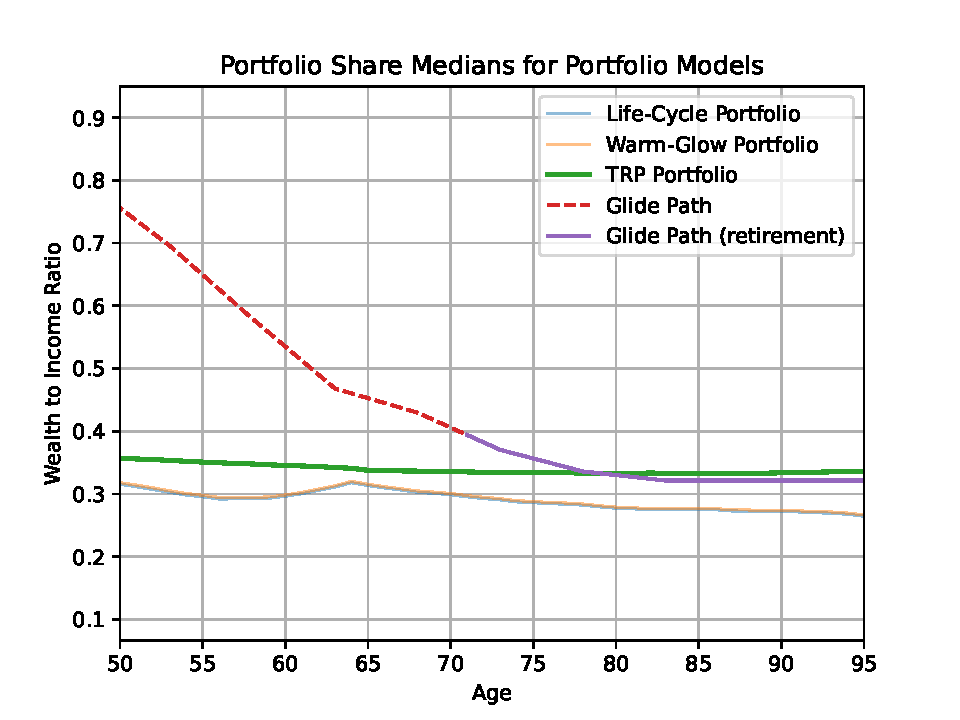
\includegraphics[width=0.7\linewidth]{files/median_share-4914e6ae678815fe96333c65f71d7d38.pdf}
\end{figure}

Some text

\begin{figure}[!htbp]
\centering
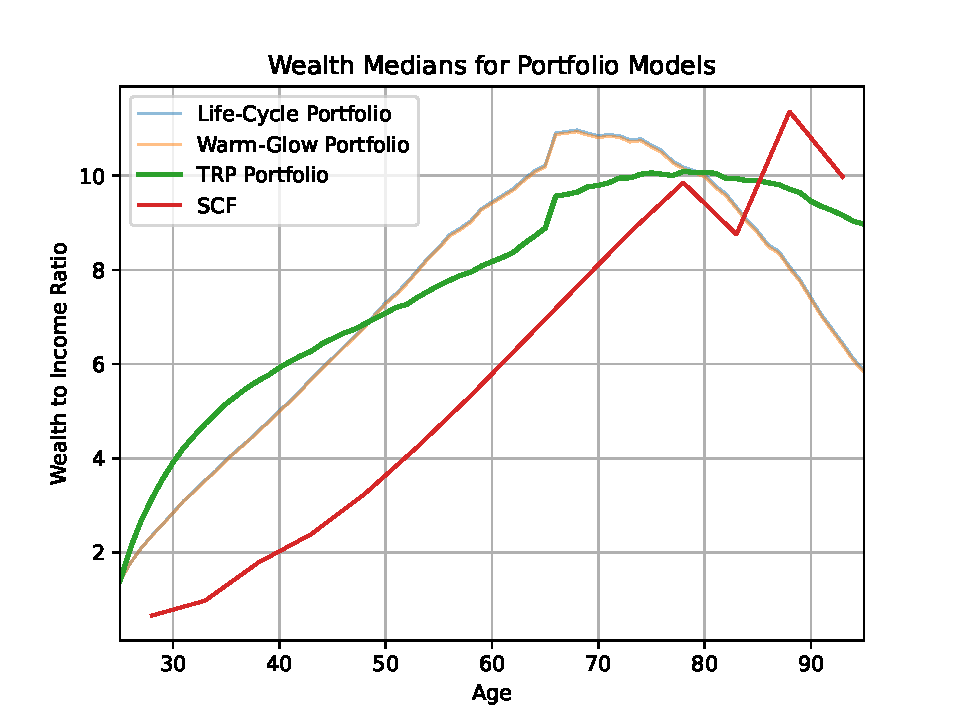
\includegraphics[width=0.7\linewidth]{files/median_wealth-54ebc582b1bc7f823c4d514c0977f5a6.pdf}
\end{figure}

\section{Conclusion}

To thoughtful academics, it has long been disturbing that the financial advice industry has paid so little attention to our hard work in constructing and solving impressively sophisticated dynamic stochastic optimization models of financial behavior. Those of us with a bit of humility have always suspected that the failure has been on our side: If all we could offer was models that produced risible advice like `everyone should spend down their wealth to zero and live pension-check to pension-check,' while financial analysts' real world experience told them that such advice would not be welcomed by their advisees, then it was reasonable to disregard the academic literature.

The thesis of this paper, though, is that a confluence of factors has now finally brought us to a point where state-of-the-art mathematical/computational optimization models can provide advice that makes sense. Much more remains to be done to improve the models further; for example, a question of great practical importance that is now just at the edge of possibility of being computationally solved is to calculate the implications of nonfinancial (principally, housing) wealth for optimal financial choice. Because homeownership is such a complex phenomenon, the academic literature is only now reaching the point at which it may be possible to answer questions like ``if I own a house, how should I modify my spending and portfolio plans to take that into account?''\footnote{We do know the \textit{direction} of the effect. \cite{kimballStandardRA} shows that the addition of a new uncontrollable risk reduces the optimal choice of exposure to controllable risks like the stock market. But \textit{by how much} one's stock exposure should be reduced because of house-price risk can only be answererd by solving a quantitatively plausible model.}

It would be a better world if financial advice could be justified as reflecting the mathematically optimal solution to a well-defined problem.  Not only would academics have the satisfaction of knowing that they had finally come close to fulfilling the vision of Modligliani and Brumberg 70 years ago. Financial analysts could also sleep more soundly in the knowledge that the advice they were giving could be what many people probably think it already is: The adaptation to the client's particular circumstances of the advice that is the best that can be delivered by the latest high-tech computational optimization tools.

The time seems ripe for a much closer collaboration between academia and the financial industry in building this better world.


\bigskip
\centerline{\rule{13cm}{0.4pt}}
\bigskip

% points to work in somewhere:

% [^fiduciary] Finally, financial advisors to 401(k) plans have a fiduciary responsibility to the employee to make prudent plans for the employee's own needs in retirement. The fiduciary duty does \emph{not} extend to heirs. To the extent that consumers follow the financial advice of their 401(k) advisor, they ought not to exhibit a bequest motive. % JT: Is there a citation I can use for this?

% [^carnegie]
% Andrew Carnegie, the richest man in the world around the turn of the 20th century, famously pledged to give away 90 percent of his wealth before his death (and made good on his promise). Carnegie was explicit: He had far more wealth than necessary to accommodate his wants (including maintenance of his beloved Scottish castle); he thought considerable social good could be accomplished by the charities he favored (especially libraries); and he felt that the expectation of receiving a colossal inheritance would 'ruin' a child.[^ruin] The reason economists should be interested in extreme examples like Carnegie (or Bill Gates, or John D. Rockefeller) is the same reason physicists are interested in black holes: Stress tests of a theory can reveal its flaws (Einstein beats Newton only in such extreme cases).
% [^ruin]: "I would as soon leave my son a curse as the almighty dollar." (Andrew Carnegie)



\bibliographystyle{unsrtnat}
\bibliography{main.bib}

\end{document}
